% Template for PLoS
% Version 1.0 January 2009
%
% To compile to pdf, run:
% latex plos.template
% bibtex plos.template
% latex plos.template
% latex plos.template
% dvipdf plos.template

% cloud in discuss at end
% point at github foo

\documentclass[10pt]{article}

% amsmath package, useful for mathematical formulas
\usepackage{amsmath}
% amssymb package, useful for mathematical symbols
\usepackage{amssymb}

% graphicx package, useful for including eps and pdf graphics
% include graphics with the command \includegraphics
\usepackage{graphicx}

% cite package, to clean up citations in the main text. Do not remove.
\usepackage{cite}

\usepackage{color} 

% Use doublespacing - comment out for single spacing
%\usepackage{setspace} 
%\doublespacing


% Text layout
\topmargin 0.0cm
\oddsidemargin 0.5cm
\evensidemargin 0.5cm
\textwidth 16cm 
\textheight 21cm

% Bold the 'Figure #' in the caption and separate it with a period
% Captions will be left justified
\usepackage[labelfont=bf,labelsep=period,justification=raggedright]{caption}

% Use the PLoS provided bibtex style
\bibliographystyle{plos2009}

% Remove brackets from numbering in List of References
\makeatletter
\renewcommand{\@biblabel}[1]{\quad#1.}
\makeatother


% Leave date blank
\date{}

\pagestyle{myheadings}
%% ** EDIT HERE **


%% ** EDIT HERE **
%% PLEASE INCLUDE ALL MACROS BELOW

%% END MACROS SECTION

\begin{document}

% Title must be 150 characters or less
\begin{flushleft}
{\Large
\textbf{These are not the k-mers you are looking for: efficient
online k-mer counting using a probabilistic data structure}
}
% Insert Author names, affiliations and corresponding author email.
\\
Qingpeng Zhang$^{1}$, 
Jason Pell$^{1}$,
Rosangela Canino-Koning$^{1}$,
Adina Chuang Howe$^{2,3}$,
C. Titus Brown$^{1,2\ast}$
\\
\bf{1} Computer Science and Engineering, Michigan State University,
East Lansing, MI, USA
\\
\bf{2} Microbiology and Molecular Genetics, Michigan State University,
East Lansing, MI, USA
\\
\bf{3} Plant, Soil, and Microbial Sciences, Michigan State University, 
East Lansing, MI, USA
\\
$\ast$ E-mail: ctb@msu.edu
\end{flushleft}

% figures: khmer blue; tallymer green; jellyfish red; dsk yellow



% @CTB mention altmetrics/popularity; top X packages?

% @CTB put in 'diff' command in Makefile
% @CTB   ref the use of Amazon for benchmarks; cloud environment.

% @CTB new stuff/TODO for submission:
% @CTB   citation combine
% @CTB   spellcheck
% @CTB   put in github tag references
% @CTB   make sure we discuss abundance dist approach

% Please keep the abstract between 250 and 300 words
\section*{Abstract}

K-mer abundance analysis is widely used for many purposes in sequence
analysis, including data preprocessing for de novo assembly, repeat
detection, and sequencing coverage estimation.
We present the khmer software package for fast and memory efficient
{\em online} counting of k-mers in sequencing
data sets. Unlike previous methods based on data structures such as
hash tables, suffix arrays, and trie structures, khmer relies entirely
on a simple probabilistic data structure, a CountMin Sketch.  The
CountMin Sketch permits online updating and retrieval of k-mer counts
in memory which is necessary to support online k-mer analysis algorithms.
On sparse data sets this data structure is considerably more memory
efficient than any exact data structure.  In exchange, the use of a
CountMin Sketch introduces a systematic overcount for k-mers;
moreover, only the counts, and not the k-mers, are stored.
Here we analyze the speed, the memory usage, and the miscount rate of khmer
for generating k-mer frequency distributions and retrieving k-mer
counts for individual k-mers.  We also compare the performance of
khmer to several other k-mer counting packages, including Tallymer,
Jellyfish, and DSK.  Finally, we examine the effectiveness of profiling 
sequencing error, k-mer abundance trimming, and
digital normalization of reads in the context of high khmer error
rates. Khmer is implemented in C++ wrapped with a Python
interface, offers a tested and robust API, and is freely available
under the BSD license at github.com/ged-lab/khmer.

% Please keep the Author Summary between 150 and 200 words
% Use first person. PLoS ONE authors please skip this step. 
% Author Summary not valid for PLoS ONE submissions.   
\section*{Author Summary}

\section*{Introduction}

The goal of k-mer counting is to determine the number of occurrences
for each fixed-length word of length k in a DNA data set
\cite{Marcais2011}. Efficient k-mer counting plays an important role
in many bioinformatics approaches, including data preprocessing for de
novo assembly, repeat detection, and sequencing coverage estimation
\cite{Kurtz2008}.

% (MRC) Shouldn't that last item have more citations?

Short-read shotgun sequencing data is both relatively sparse in
k-mers and contains many erroneous k-mers.  For typical values of k such 
as 32 the data sets are sparse as only a small fraction of
the total possible number of k-mers ($4^{32}$) are actually present in
any genome or read data sets derived from the genome.  The 
high error rate (e.g. Illumina has a ~0.1-1\%
per-base error rate \cite{pubmed19997069}) generates many unique k-mers. 
As the total number of generated reads increases, the
total number of errors grows with it linearly. This leads to data sets where the
erroneous k-mers vastly outnumber the true k-mers \cite{Conway2011}.
Tracking and counting the resulting large number of k-mers, most of
which are erroneous, has become an unavoidable and challenging task
in sequence analysis
\cite{Minoche2011}.

A variety of k-mer counting approaches, and standalone software
packages implementing them, have emerged in recent years; this
includes Tallymer, Jellyfish, BFCounter, DSK, KMC, and Turtle \cite{Kurtz2008,
Marcais2011, Melsted2011, Rizk2013, Deorowicz2013, Roy2013}.
% @CTB see http://arxiv.org/abs/1305.1861)
% @CTB include more discussion of BFcounter & turtle? What about KMC?
These
approaches and implementations each offer different algorithmic
trade-offs and enable a non-overlapping set
of functionality.  Tallymer uses a suffix tree to store k-mer counts
in memory and on disk.  Jellyfish stores k-mer counts in in-memory
hash tables, and makes use of disk storage to scale to larger
data sets.  BFCounter uses a Bloom filter as a pre-filter to avoid
counting unique k-mers, and is the first published probabilistic approach
to k-mer counting.  DSK adopts a streaming approach to k-mer counting that
enables time- and memory-efficient k-mer counting with an explicit
trade-off between disk and memory usage.  KMC relies primarily
on fast and inexpensive disk access to count k-mers in low
memory.  Turtle provides several different containers that offer
different false positive and false negative tradeoffs when counting k-mers.

Our motivation for exploring efficient k-mer counting comes from our
work with metagenomic data, where we routinely encounter data sets
that contain $300 \times 10^9$ bases of DNA and over 50 billion
distinct k-mers \cite{Howe2012}.  To efficiently filter,
partition, and assemble these data, we need to store counts for each
of these k-mers in main memory, and query and update them in realtime
--- a set of functionality not readily offered by current packages.
Moreover, we wish to enable the use of cloud and desktop
computers, which may have poor I/O performance or limited memory. These
needs have
dictated our exploration of efficient in-memory k-mer counting
techniques.

% (MRC) Three dashes for setting of a section of text

Below, we describe an implementation of a simple probabilistic data
structure for k-mer counting.  This data structure is based on a
CountMin Sketch, a generalized probabilistic data structure for
storing the frequency distributions of distinct elements
\cite{Cormode2005}.  Our implementation extends an earlier
implementation of a Bloom filter, which has been previously used for
both k-mer counting and de Bruijn graph storage and traversal
\cite{Bloom70,BroderM03,Melsted2011,Pell2012,Rizk2013,Jones:2012aa}

Probabilistic approaches can be particularly memory efficient for
certain problems, with memory usage significantly lower than any exact
data structure \cite{Pell2012}.  However, their use introduces set
membership or counting false positives, which have effects that must
be analyzed in the context of specific problems.  Moreover, unlike
existing techniques, the CountMin Sketch stores only counts;
k-mers must be retrieved from the original data set.  In exchange,
the low memory footprint enabled by this probabilistic approach enables
online updating and retrieval of k-mer counts entirely in memory, which
in turn supports streaming applications such as digital normalization
\cite{Brown2012}.

% @CTB cloud in discusson at end
We use the Amazon cloud to compare time, memory, and disk usage of our k-mer counting
implementation with that of Tallymer, Jellyfish, and DSK, for two problems. First, we 
generate a k-mer abundance distribution for large
data sets; and second, we query many individual k-mer counts at random from
a previously constructed k-mer count database.  We show that khmer
is competitive in speed, memory, and disk usage for these
problems.  We also analyze the effects of counting error on
calculations of the k-mer count in sequencing data sets,
and in particular on metagenomic data sets.  Finally, we discuss
khmer's miscount performance in the context of two specific applications:
low-abundance k-mer trimming of reads, and digital normalization.

% (MRC) Is this a comparison paper or a khmer-is-capable-of-many-things paper?

The khmer software is implemented in C++ with a Python wrapper,
enabling flexible use and reuse by users with a wide range of
computational
expertise.  The software package is freely available for academic and
commercial use and redistribution under the BSD license at
github.com/ged-lab/khmer/.  khmer comes with substantial documentation
and many tutorials, and contains extensive unit tests.  Moreover, we
have built several applications on top of khmer, including
memory-efficient de Bruijn graph partitioning \cite{Pell2012} and
lossy compression of short-read data sets for assembly
\cite{Brown2012}.

% Results and Discussion can be combined.
\section*{Results}

\subsection*{Implementing a CountMin Sketch for k-mers}

The two basic operations supported by khmer are {\tt c =
  increment\_count(kmer) } and {\tt c = get\_count(kmer). }
Both operate on the data structure in memory, such that neither
incrementing a count nor retrieving a count involves disk
access.

The implementation details are similar to those of the Bloom filter in
\cite{Pell2012}, but with the use of 8 bit counters instead of 1 bit
counters.  Briefly, Z hash tables are allocated, each with a different
size of approximately H bytes (H\_1, H\_2, ..., H\_Z); the sum of these hash table sizes must
fit within available main memory.  To increment the count for a
particular k-mer, a single hash is computed for the k-mer, and the
modulus of that hash with each hash table's size H gives the location
for each hash table; the associated count in each hash table is then
incremented by 1.  We use different size for each hash table so 
the locations in different hash tables for that particular k-mer will be different. 
If two k-mers have a collision in one hash table which means the locations given by the modulus calculation
are the same, chances are that the two k-mers will not have collision in another hash 
table with different size.
To retrieve the count for a k-mer, the same hash is
computed and the minimum count across all hash tables is computed.
While different in implementation detail from the standard CountMin Sketch,
which uses a single hash table with many hash
functions, the performance details are identical \cite{Pell2012}.

An additional benefit of the CountMin Sketch is that it is extremely
easy to implement correctly, needing only about 3 dozen lines of C++
code for a simple threadsafe implementation.

To determine the expected error rate --- the average frequency
with which a given k-mer count will be incorrect when retrieved --- we
can look at the hash table load. Suppose N unique k-mers have been
counted using Z hash tables, each with size H.  The probability that
no collisions happened in a specific entry in one hash table is
$(1-1/H)^{N}$, which can be approximated as $e^{-N/H}$. The individual
collision rate in one hash table is $1-e^{-N/H}$. The total collision
rate, which is the probability that a collision occurred in each entry
where a k-mer maps to in all Z hash tables, is $(1-e^{-N/H})^{Z}$.

While the error rate can easily be calculated from the hash
table load, the average {\em miscount} --- the degree to which the measured count
differs from the true count --- depends on the k-mer frequency
distribution, which must be determined empirically.  We analyze the
effects of this below.

\subsection*{khmer efficiently calculates k-mer abundance histograms}

We measured time and memory required to calculate k-mer abundance
histograms in five soil metagenomic read data sets using khmer,
Tallymer, Jellyfish, and DSK (Table \ref{table:datasets}; Figures \ref{fig:cmp_time} and
\ref{fig:cmp_memory}).  We chose to benchmark abundance histograms because
this functionality is common to all four software packages, and is a
common analysis approach for determining assembly parameters \cite{Chikhi:2014aa}.
We applied each package to increasingly large subsets of a 50m read soil
metagenome data set \cite{Howe2012}.

Figure \ref{fig:cmp_time} shows that the time usage of our khmer approach
is comparable to Jellyfish and DSK, and, as expected, increases linearly
with data set size. Tallymer is the slowest of the four tools in this testing.

From Figure \ref{fig:cmp_memory}, we see that the memory usage of both
Jellyfish and Tallymer increases linearly with data set size. Tallymer uses more 
memory than Jellyfish generally.  DSK uses less memory
than all of the other programs for large data sets, but at the cost
of more limited functionality (discussed below).

In addition, the memory usage of khmer also increases linearly with
data set size as long as we hold the error rate constant.  However,
the memory usage of khmer varies substantially with the desired error
rate: we can decrease the memory usage by increasing the
error rate, as shown in Figure \ref{fig:cmp_memory}.  We also
see that with a low error rate of 1\%, the
memory usage is competitive with Tallymer and Jellyfish; with a higher 5\%
error rate, the memory usage is lower than all but the
disk-based DSK; with an error rate as 20\%, the memory usage is further lower,
close to DSK.

The memory usage of Jellyfish is dependent on the k-mer
size, because it uses hash tables to store k-mer counts and must store
the exact k-mer to track collisions; however, khmer's memory
usage is independent of k, because it does not track collisions.

We also measured disk usage during counting.
Figure \ref{fig:cmp_disk} shows that
the disk usage also increases linearly with the number of k-mers in the
data set.
For a high-diversity metagenomics
data set of 5 GB, the disk usage of both Jellyfish and Tallymer is
around 30 GB.  khmer counts k-mers entirely in working memory and does
not rely on any on-disk storage to store or retrieve k-mer counts,
although for practicality the hash tables can be saved for later
reuse; the uncompressed disk usage for khmer in Figure \ref{fig:cmp_disk}
is the same as its memory.  At the expense of more time, khmer
supports saving and loading gzip-compressed hash tables, which are
competitive in size to DSK's on-disk database (Figure 3, dashed line).

\subsection*{khmer accesses k-mer counts efficiently}

We measured the time it took to access 9.7m 22-mers across five
different data sets after the initial databases had been built (Figure
\ref{fig:cmp_count}).  Note that Tallymer, Jellyfish, and khmer all
support random access to k-mer counts, while DSK does not. Here,
khmer and Tallymer performed well, dramatically outperforming
Jellyfish.  In all three cases, system time dominated the overall time
required to retrieve k-mers, suggesting that the primary reason for
the linear increase in retrieval time was due to the increased size of
the database on the disk (data not shown).  In particular, khmer is
 independent of the size of the database in retrieval time once the hash tables are loaded into
memory.

\subsection*{The measured counting error rate is low on short-read data}

Due to the use of CountMin Sketch and its lack of collision tracking,
khmer will report some incorrect counts for k-mers; these counts are
always higher than the true counts if within bound of 255 which is limited by 
the 8-bit counters we used. The frequency with which 
 incorrect counts are reported can be estimated from the hash table
load.  However, the expected {\em miscount} --- the difference
between the true k-mer frequency and the reported k-mer frequency --- cannot be
calculated without knowing the distribution of k-mer abundances; in
general, the average miscount will be small if the data is
left-skewed.  As noted by Melsted and Pritchard, a large number of k-mers in
short-read data are low-abundance, leading to precisely the skew
that would yield low miscounts \cite{Melsted2011}.  Here we use both
real and simulated data sets to evaluate the counting performance in
practice.

Figure \ref{fig:average_offset_vs_fpr} shows the relationship between
average miscount and counting error rate for five different test data
sets with similar numbers of distinct k-mers: one metagenome data
set; a simulated set of random k-mers; a simulated set of reads,
chosen with 3x coverage and 1\% error; a simulated set of reads (3x)
with no error and a set of {\em E. coli} reads (Table \ref{table:random_data}).  
Even when the counting error rate is as high as 0.9 ---
where 90\% of k-mers have an incorrect count --- the average miscount is still
below 4.

We separately analyzed the average {\em percentage} miscount between
true and false k-mers; e.g. an miscount of 4 for a k-mer whose true
count is 1 would be 400\%.  Figure \ref{fig:percent_offset_vs_fpr} shows 
the relationship between average miscount and counting error rate for 
the same five data sets as in Figure \ref{fig:average_offset_vs_fpr}.  
For an error rate of 0.1 (10\% of k-mer counts are incorrect), 
the average percentage miscount is less than 10\% for all five data 
sets; this will of course generally be true, 
because the average miscount is bounded by the product of the error 
rate times k-mer abundance.

We see here that for a fixed counting error rate, the simulated reads
without error have the highest average miscount, and the randomly generated
k-mers have the lowest average miscount.  This is because these two
abundance distributions have the least and most left-skew,
respectively: the simulated reads without error have no abundance-1
k-mers, while the randomly generated k-mers are entirely low abundance.
% E.coli reads dataset has lower "coverage" than simulated reads without error.

\subsection*{Sequencing error profiles can be measured with k-mer abundance
profiles}

One specific use for khmer is detecting random sequencing errors by
looking at the k-mer abundance distribution within reads \cite{Medvedev2011}.
Low-abundance k-mers contained in a high-coverage data set typically
represent random sequencing errors, and a variety of read trimming and
error correcting tools use k-mer counting to reduce the error content
of the read data set, independent of quality scores or reference
genomes \cite{Kelley2010}.  This is an application where the counting
error of the CountMin Sketch approach used by khmer may be
particularly tolerable: it will never falsely call a high-abundance k-mer 
as low-abundance because khmer never underestimates counts.


In Figure \ref{fig:perc_unique_pos}, we use khmer to examine the
sequencing error pattern of a 5m-read subset of an Illumina reads
data set from single-colony sequencing of {\em E. coli}
\cite{pubmed21926975}.  The high rate of occurrence of unique k-mers
close to the 3' end of reads is due to the increased error rate at the
3' end of reads.

\subsection*{khmer can be applied iteratively to read trimming}

One approach to error reduction in short-read data sets is to trim
reads at low-abundance k-mers, which in high-coverage genome
sequencing data sets are largely due to sequencing errors \cite{Kelley2010}.
Here counting errors from khmer result in a one-sided trimming
error such that some low-abundance k-mers are retained, but no
high-abundance k-mers are erroneously trimmed; low-abundance k-mer
trimming can easily be applied iteratively, with increasing accuracy
at each iteration.

% @CTB discuss application to larger genomes in discussion
We performed four iterations of unique k-mer trimming on 5 million
Illumina reads from sequencing of {\em E. coli}, with a maximum memory
usage of 40 MB.  For each iteration we measured empirical error rate
compared with number of bases trimmed as well as the total number of
k-mers
(Table \ref{table:loop_trim}).
In the first round, the estimated error
rate was 78.1\%, and 22\% of the total bases were removed by trimming
reads at low-abundance k-mers; the second iteration had an error
rate of 10\%, and removed only 2.9\% additional data; and by
the fourth iteration the error rate was down to 3.1\% with 0.0\% of the data removed.

The elimination of so many unique k-mers (column 5) in the first pass
was unexpected: the high error rate should have resulted in
fewer unique k-mers being identified as unique, were the erroneous
k-mers independent of each other. Upon examination, we realized that
in Illumina data erroneous k-mers typically come from substitution
errors that yield runs of up to k erroneous k-mers in a row \cite{Kelley2010}.  
When trimming reads with high error rates,
these runs are typically trimmed after the first few unique k-mers,
leaving unique k-mers at the 3' end.
Because of this we hypothesized that high-FP rate trimming would
result in the retention of many unique k-mers at the 3' end of the
read, and this was confirmed upon measurement (Table \ref{table:loop_trim}, column 6, 
pass 1 vs pass 2).

\subsection*{Using khmer for digital normalization, a streaming algorithm}

Digital normalization is a lossy compression algorithm that discards
short reads based on saturating coverage of a de Bruijn graph
\cite{Brown2012}.  While several non-streaming implementations exist, including
Trinity's {\em in silico} normalization \cite{Haas2013,Brown2012blog}, digital 
normalization can be efficiently implemented as a {\em
  streaming} algorithm. The first pass of the three-pass procedure
of digital normalization involves reading in all of the reads, so it is by far the most
computationally intensive. If a read is determined to be discarded,
it will not be loaded into the CountMin Sketch structure. So the majority of k-mers in a data set
are never loaded into the counting structure and the next two passes will be
much more efficient. This has the advantage of enabling 
low-memory preprocessing of both high-coverage genomic data sets and mRNAseq or
metagenomic data sets with high-coverage components \cite{Brown2012,
  Howe2012}.  While digital normalization is already
implemented inside khmer, previous work did not explore the lower bound
on memory usage for effective digital normalization.

% @CTB how do we calculate MOST EFFICIENT arrange of -N and -x?
We applied digital normalization to the {\em E. coli} data set used
above; choosing three different CountMin Sketch sizes yielded three different
error rates: 40 MB RAM (82.9\%), 80 MB RAM (39.3\%), and 800 MB RAM
(0.00\%).  Data sets were normalized to a k-mer coverage of 20 and the
resulting data were evaluated for retention of true and erroneous
k-mers, as in \cite{Brown2012} (Table \ref{table:loop_norm}).  The results show that
digital normalization retains the same set of underlying
k-mers even at the highest error rate (Table \ref{table:loop_norm}, column 3), 
while discarding only about 2\% additional reads (Table \ref{table:loop_norm}, column 4).

To evaluate the effect on actual genome assembly, we next performed
error trimming and normalization to a coverage of 5 (the
``three-pass'' protocol from \cite{Brown2012} recommended for
genome assembly), staying within the specified memory bounds.  We then
assembled this data with Velvet \cite{Zerbino2008} and compared the resulting 
assemblies to the known {\em E. coli} MG1655 genome (Table \ref{table:assembly}. 
In terms of overall size and genome content, all three assemblies were nearly identical 
(table \ref{table:assembly}, column 4).  Thus digital normalization is surprisingly 
refractory to high error rates even for practical assembly outcomes.  (Note that
the Velvet assembler itself used considerably more memory than digital
normalization.)







\section*{Discussion}


\subsection*{khmer enables fast, memory-efficient online counting}

khmer enables memory- and time-efficient online counting (Figures \ref{fig:cmp_time}, 
\ref{fig:cmp_memory}, and \ref{fig:cmp_count}).  This is
particularly important for the streaming approaches to data analysis
needed as data set sizes increase.  Because query and updating of
k-mer counts can be done directly as data is being loaded, with no
need for disk access or an indexing step, khmer can also perform
well in situations with poor disk I/O performance.  (Note that BFCounter
also supports online k-mer counting, but is not currently competitive
in speed \cite{Deorowicz2013}.)

\subsection*{khmer is a generally useful k-mer counting approach}

In addition to online counting, khmer offers a general range of useful
performance tradeoffs for disk I/O, time and memory.  From the
performance comparison between khmer and other k-mer counting packages
in calculating k-mer abundance distributions, khmer is comparable with
existing packages.  In time, khmer performs competitively with DSK and
Jellyfish (Figure \ref{fig:cmp_time}); khmer also provides a way to systematically trade 
memory for miscounts across a wide range of parameters (Figure \ref{fig:cmp_memory}).  khmer's
uncompressed disk storage is competitive with Jellyfish, and, in
situations where disk space is at a premium, khmer can take advantage
of gzip compression to provide storage similar to that of DSK (Figure \ref{fig:cmp_disk}, 
dashed blue line).

Interestingly, DSK performs especially well in memory usage
for calculating the abundance distribution of k-mers. However, in
exchange for this efficiency, retrieving specific k-mer counts at
random is likely to be quite slow, as DSK is optimized for iterating
across partition sets of k-mers rather than randomly accessing k-mer
counts.

For retrieving the counts of individual k-mers, khmer is significantly faster than both
Tallymer and Jellyfish.  This is not surprising, since this was a
primary motivation for the development of khmer.
% @CTB check this ``significantly faster'' after running in cloud.

\subsection*{khmer memory usage is fixed and low}

The memory usage of the basic CountMin Sketch approach is fixed, which
means that khmer will never crash due to memory limitations, and all
operations can be performed in main memory without recourse to disk
storage.  However, the memory size must be chosen in light
of the error rate and miscount acceptable for a given
application.

For any given data set, the size and number of hash tables will
determine the accuracy of k-mer counting with khmer.  Thus, the user
can control the memory usage based on the desired level of
accuracy (Figure \ref{fig:cmp_memory}). The time usage for the first step of k-mer counting,
consuming the reads, depends on the
total amount of data, since we must traverse every k-mer in every read.
The second step, k-mer retrieval, is algorithmically constant for
fixed k; however, for practicality, the hash tables are usually saved
to and loaded from disk, meaning that k-mer retrieval time depends directly
on the size of the database being queried.

The memory usage of khmer is particularly low for sparse data sets,
especially since only main memory is used and no disk space is
necessary beyond that required for the read data sets.  This is no
surprise: the information theoretic comparison in
\cite{Pell2012} shows that, for sparse sequencing data sets, Bloom
filters require considerably less memory than any possible exact
information storage for a wide range of error rates and data set
sparseness.

In our implementation we use 1 byte to store the count of each k-mer
in the data structure. Thus the maximum count for a k-mer will be 255.
In cases where tracking bigger counts is required, khmer also provides
an option to use an STL map data structure to store counts above 255,
with the trade-off of significantly higher memory usage.  In the
future, we may extend khmer to counters of arbitrary bit sizes.

% @CTB discuss flexible container paper

\subsection*{Error rates in k-mer counting are low and predictable}

The CountMin Sketch is a probabilistic data structure with a
one-sided error that results in random overestimates of k-mer
frequency, but does not generate underestimates. The chosen parameters
of the data structure will influence the accuracy of the count.  While
the probability of an inaccurate count can easily be estimated based
on the hash table load, the miscount size is dependent on details of
the frequency distribution of k-mers \cite{Cormode2005}.

More specifically, in the analysis of the CountMin
Sketch, the miscount between the incorrect count and
actual count is related to the total number of k-mers in a data set and
the size of each hash table \cite{Cormode2005}. Further study has shown that the behavior
of CountMin Sketch depends on specific characteristics of the data
set under consideration, especially left-skewness \cite{Rusu2008,
  CormodeM05}.  These probabilistic properties suit short reads
from next generation sequencing data sets: the miscounts are
low because of the
highly left-skewed abundance distribution of k-mers in these data sets.

Figures \ref{fig:average_offset_vs_fpr} and \ref{fig:percent_offset_vs_fpr}
demonstrate these properties well.  We see more correct
counting for error-prone reads from a genome than for error-free
reads from a genome, with a normal
distribution of k-mer abundance.  Thus, this counting approach is
especially suitable for high diversity data sets, such as metagenomic
data, in which a larger proportion of k-mers are low abundance or
unique due to sequencing errors.

\subsection*{Real-world applications for khmer}

For many applications, an approximate k-mer count is sufficient.  For
example, when eliminating reads with low abundance k-mers, we
can tolerate a certain number of low-frequency k-mers remaining in
the resulting data set falsely.  If RAM-limited we can do the
filtering iteratively so that at each step we are making more
effective use of the available memory.

In practice, we have found that an error rate of between 1\%
and 10\% offers acceptable miscount performance for a wide range of
tasks, including error profiling, digital normalization and
low-abundance read-trimming.  Somewhat surprisingly, error
rates of up to 80\% can still be used for both read trimming and
digital normalization in memory-limited circumstances, although
multiple passes across the data may be needed.

For many applications, the fact that khmer does not break an imposed
memory bound is extremely useful, since for many data sets ---
especially metagenomic data sets --- high memory demands constrain analysis 
\cite{Howe2012,Luo2009}.  Moreover, because the error
rate is straightforward to measure, the user can be warned that the
results should be invalidated when too little memory is used.  When combined
with the graceful degradation of performance for both error trimming
and digital normalization, khmer readily enables analysis of extremely
large and diverse data sets \cite{adina2013} In an experiment to assemble 
the reads of a soil metagenomic sample collected from Iowa prairie, the number 
of reads to assemble drops from 3.3 million to 2.2 million and the size of data set
drops from 245GB to 145GB accordingly after digital normalization  \cite{Howe2012}. 
240GB memory was used in the process.This also shows khmer works well to 
analyze real-world large metagenomic data sets.

\subsection*{Conclusion}

K-mer counting is widely used in bioinformatics, and as sequencing data set sizes
increase, graceful degradation of data structures in the face of large
amounts of data has become important.  This is especially true when
the theoretical and practical effects of the degradation can be
predicted (see e.g. \cite{Melsted2011, Pell2012, Roy2013}).  This
is a key property of the CountMin Sketch
approach, and its implementation in khmer.

The khmer software implementation offers good performance, a robust
and well-tested Python API, and a number of useful and well-documented
scripts.  While Jellyfish and DSK also offer good performance,
khmer is competitive, and, because it provides a
Python API for online counting, is flexible.  In memory-limited
situations with poor I/O performance, khmer is particularly useful,
because it will not break an imposed memory bound and does not require
disk access to store or retrieve k-mer counts.  However, in exchange
for this memory guarantee, counting becomes increasingly incorrect as
less memory is used or as the data set size grows large; in many
situations this may be an acceptable tradeoff.

\subsection*{Future considerations}

Applying khmer to extremely large data sets with many unique k-mers
requires a large amount of memory: approximately 446 GB of memory is
required to achieve an error rate of 1\% for
$50\times 10^9$ k-mers. It is possible to reduce the required memory by dividing
k-mer space into multiple partitions and counting k-mers separately
for each partition. Partitioning k-mer space into $M$ partitions
results in a linear decrease in the number of k-mers under
consideration, thus reducing the occupancy by a constant factor $M$
and correspondingly reducing the collision rate.  Partitioning k-mer
space is a generalization of the systematic prefix filtering approach,
where one might first count all k-mers starting with AA, then AC, then
AG, AT, CA, etc., which is equivalent to partitioning k-mer space into
16 equal-sized partitions. These partitions can be calculated
independently, either across multiple machines or iteratively on a
single machine, and the results stored for later comparison or
analysis.  This is similar to the approach taken by DSK
\cite{Rizk2013}, and could easily be implemented in khmer.

Further optimization of khmer on single machines, e.g. for multi-core
architectures, is unlikely to achieve significantly greater speed.
Past a certain point k-mer counting is fundamentally I/O bound
\cite{McDonald2013}.

Perhaps the most interesting future direction for probabilistic k-mer
counting is that taken by Turtle \cite{Roy2013}, in which several
data structures are provided, each with different tradeoffs, but with
a common API.  We hope to pursue this direction in the future by
integrating such approaches into khmer.
% see: http://delivery.acm.org.proxy1.cl.msu.edu/10.1145/2490000/2487357/p123-huang.pdf?
% ip=35.8.11.2&acc=ACTIVE%20SERVICE&key=C2716FEBFA981EF16B5540ABA7506E55713C06D93B9F76B9
% &CFID=344104418&CFTOKEN=64899208&__acm__=1372542398_54d84e5dea52f6a71c5b8e462040a819

\section*{Methods}

\subsection*{Code and data set availability}

% @CTB update

The version of khmer used to generate the results below is available
at http://github.com/ged-lab/khmer.git, tag '2013-khmer-counting'.
Scripts specific to this paper are available in the paper repository
at https://github.com/ged-lab/2013-khmer-counting.
The IPython\cite{4160251} notebook file and data analysis to generate the figures are also
available in that github repository.  Complete instructions to reproduce
all of the results in this paper are available in the khmer-counting
repository; see tutorial.rst.

\subsection*{Sequence Data}

One human gut metagenome reads data set (MH0001) from the 
MetaHIT (Metagenomics of the Human Intestinal Tract) project \cite{Qin2010} was used. 
It contains approximately 59 million reads, each 44bp long; it was trimmed to remove 
low quality sequences. 

Five soil metagenomics reads data sets with different size were taken
from the GPGC project for benchmark purpose (see Table
\ref{table:datasets}).  These reads are from soil in Iowa region and they
are filtered to make sure there are less than 30\% Ns in the read and
each read is longer than 30 bp.  The exact data sets used for the
paper are available on Amazon S3 and the instructions to acquire these
data sets are available in the paper repository on github.com.

We also generated four short-read data sets to assess the error
rate and miscount distribution. One is a subset of a real
metagenomics data set from the MH0001 data set, above. The second
consists of randomly generated reads. The third and fourth contain
reads simulated from a random, 1 Mbp long genome.  The third has a
substitution error rate of 3\%, and the fourth contains no errors. The
four data sets were chosen to contain identical numbers of unique
22-mers.  The scripts necessary to regenerate these data are available
in the paper repository on github.com.

\subsection*{CountMin Sketch implementation}

We implemented the CountMin Sketch data structure, a simple
probabilistic data structure for counting distinct elements
\cite{Cormode2005}.  Our implementation uses $Z$ independent hash
tables, each containing a prime number of counters $H_i$.  The hashing
function for each hash table is fixed, and reversibly converts each
DNA k-mer (for $k \le 32$) into a 64-bit number to which the modulus of
the hash table size is applied.  This provides $Z$ distinct hash
functions (see also \cite{adina2013}).

To increment the count associated with a k-mer, the counter associated
with the hashed k-mer in each of the $N$ hash tables is incremented.
To retrieve the count associated with a k-mer, the minimum count
across all $N$ hash tables is chosen.

In this scheme, collisions are explicitly not handled, so the count
associated with a k-mer may not be accurate. Because collisions only
falsely {\em increment} counts, however, the retrieved count for any
given k-mer is guaranteed to be no less than the correct count.  Thus
the counting error is one-sided.

\subsection*{Hash function and khmer implementation}

The current khmer hash function works only for $k \le 32$ and converts
DNA strings exactly into 64-bit numbers.  However, any hash function
would work. For example, a cyclic hash would enable khmer to count
k-mers larger in size than 32; this would not change the scaling
behavior of khmer at all, and is a planned extension.

By default khmer counts k-mers in DNA, i.e. strandedness is
disregarded by having the hash function choose the lower numerical
value for the exact hash of both a k-mer and its reverse complement.
This behavior is configurable via a compile-time option.

\subsection*{Comparing with other k-mer counting programs}

We generated k-mer abundance histograms from five soil metagenomic reads
data sets of different sizes using khmer, Tallymer, Jellyfish, and DSK.
We fixed k at 22 unless otherwise noted.

\paragraph{khmer:}
For khmer, we set hash table sizes to fix the error rate at
either 1\%, 5\% or 20\%, and used 8 threads in loading the data.

We did the khmer random-access k-mer counting benchmark with a
custom-written Python script {\tt khmer-count-kmers} which loaded the
database file and then used the Python API to query each k-mer
individually.

\paragraph{Tallymer:}
Tallymer is from the genometools package version 1.3.4. For the suffixerator subroutine 
we used:
{\tt -dna -pl -tis -suf -lcp -parts 4}.

For the mkindex subroutine, we used: {\tt -mersize 31} and {\tt -mersize 22}.

The Tallymer random access k-mer counting benchmark was done using the
'tallymer search' routine against both strands; see the script
{\tt tallymer-search.sh}.

\paragraph{Jellyfish:}
Jellyfish is version 1.1.2 and the multithreading option is set to 8 threads.

Jellyfish uses a hash table to store the k-mers and the size of the
hash table can be modified by the user.  When the specified hash table
fills up, Jellyfish writes it to the hard
disk and initializes a new hash table.  Here we use a
similar strategy as in \cite{Melsted2011} and chose the minimum size of the hash 
tables for Jellyfish so that all k-mers were stored in memory.

We ran Jellyfish with the options as below:

{\tt jellyfish count -m 22 -c 2 -C} for k=22.

{\tt jellyfish count -m 31 -c 2 -C} for k=31.

The Jellyfish random access k-mer counting benchmark was performed
using the 'query' routine and querying against both strands; see
the script {\tt jelly-search.sh}.

\paragraph{DSK:} We ran DSK with default parameters.


% Do NOT remove this, even if you are not including acknowledgments
\section*{Acknowledgments}

We thank Eric McDonald for technical assistance with optimizing the khmer codebase.


%This work was supported in part by the USDA (XXXX-XXXX), NSF (), BEACON, MBL
%


%\section*{References}
% The bibtex filename
\bibliography{khmer-counting-revision}
\clearpage

\section*{Figure Legends}

%\begin{figure}[!ht]
%\begin{center}
%%\includegraphics[width=4in]{figure_name.2.eps}
%\end{center}
%\caption{
%{\bf Bold the first sentence.}  Rest of figure 2  caption.  Caption 
%should be left justified, as specified by the options to the caption 
%package.
%}
%\label{Figure_label}
%\end{figure}


%\graphicspath{./figure/}

% @CTB explain why different runs
\begin{figure}[!ht]
\centerline{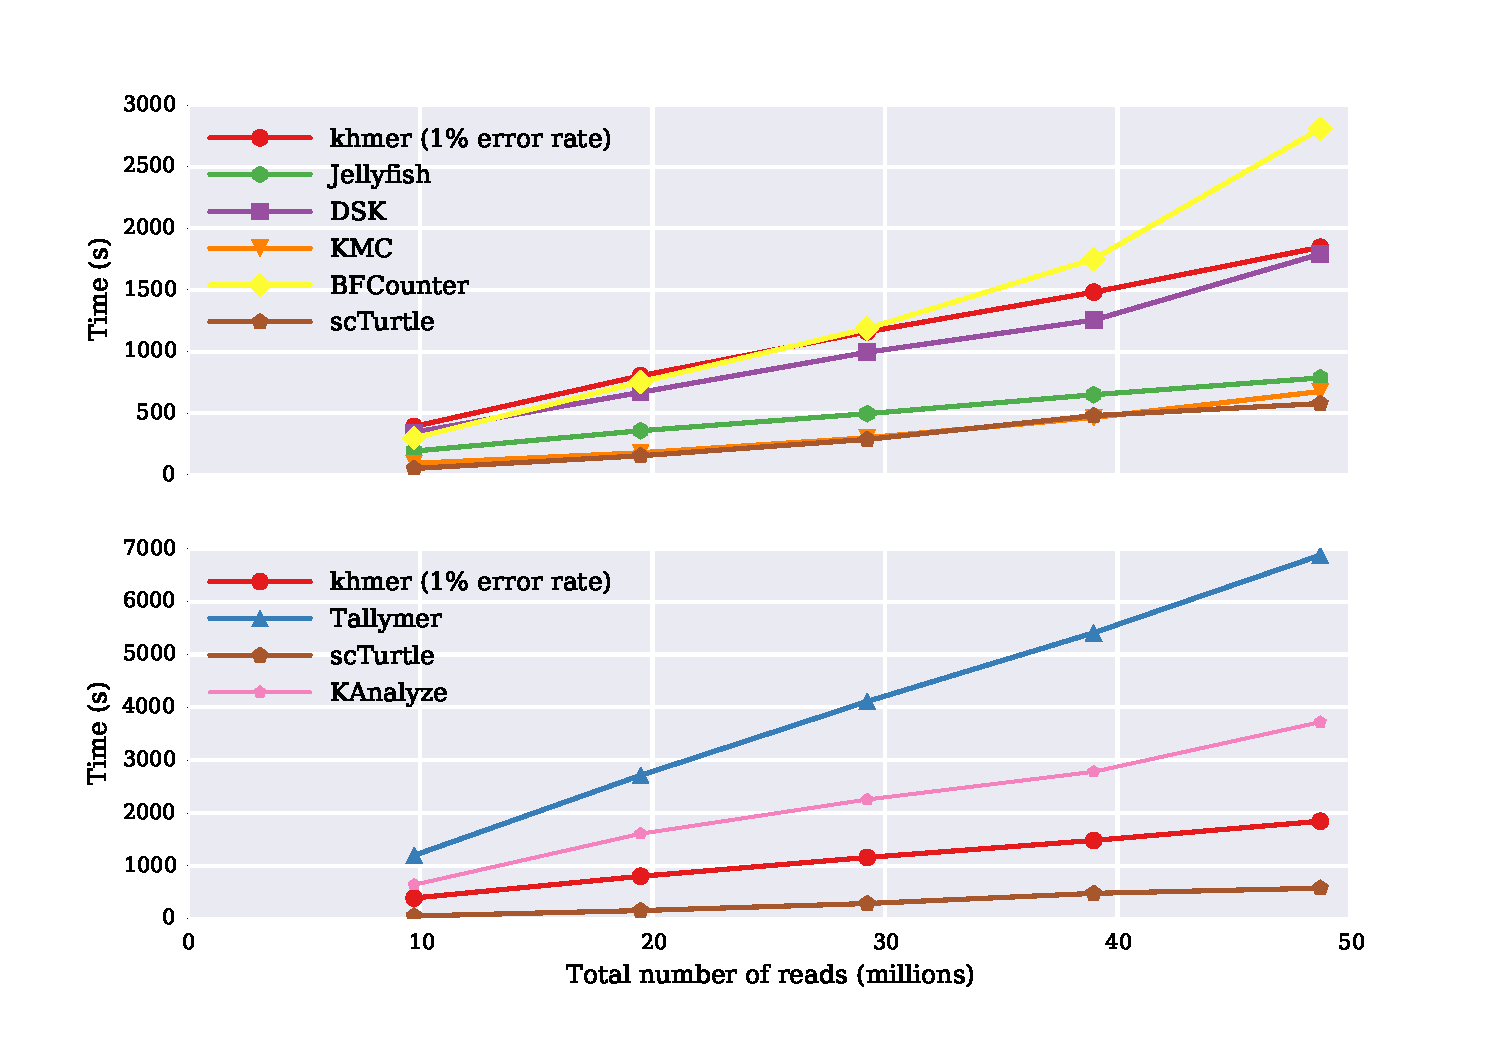
\includegraphics[width=5in]{./figure/time_benchmark}}
\caption{\bf Time usage of four different k-mer counting tools to calculate k-mer 
abundance histograms(y axis, in seconds) against data set size (in reads number, x axis).}
\label{fig:cmp_time}
\end{figure}

\begin{figure}[!ht]
\centerline{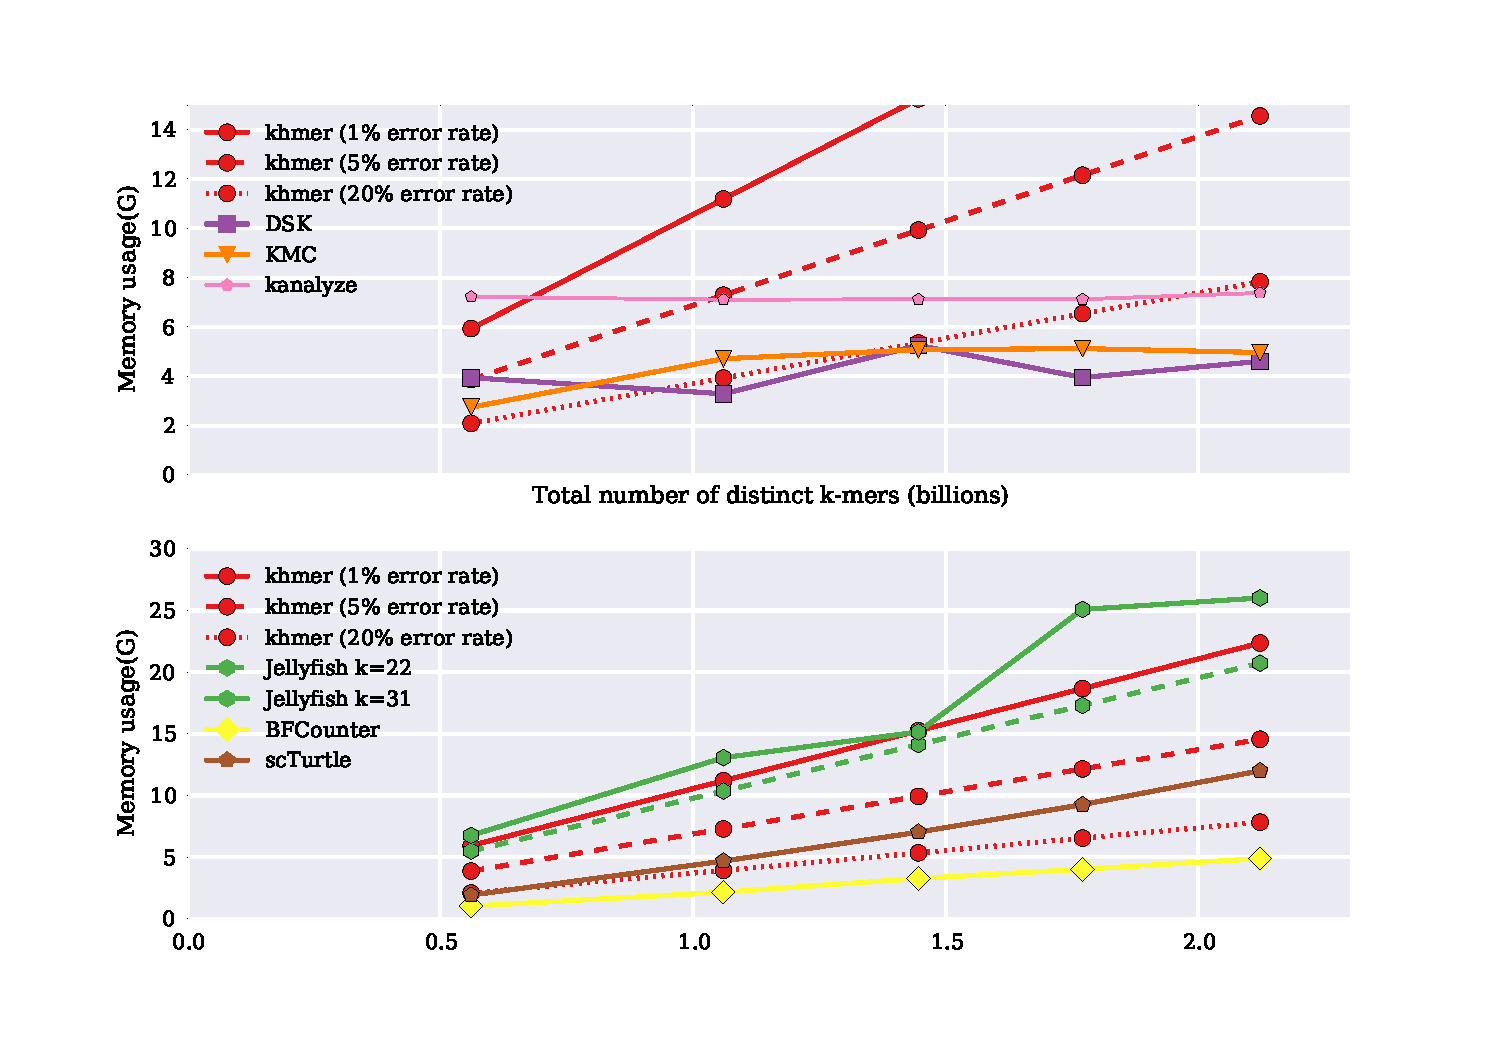
\includegraphics[width=5in]{./figure/memory_benchmark}}
\caption{\bf Memory usage of different k-mer counting tools to calculate k-mer abundance 
histograms(y axis, maximum resident program size, GB) plotted against the total number 
of distinct k-mers in the data set, for typical program settings. DSK uses the disk to 
store k-mers and is therefore constant in memory use. By increasing the error rate in 
khmer, memory usage can be substantially decreased (compare solid blue line with dashed 
and dotted blue line). K-mer size is 22 except otherwise mentioned.}
\label{fig:cmp_memory}
\end{figure}

\begin{figure}[!ht]
\centerline{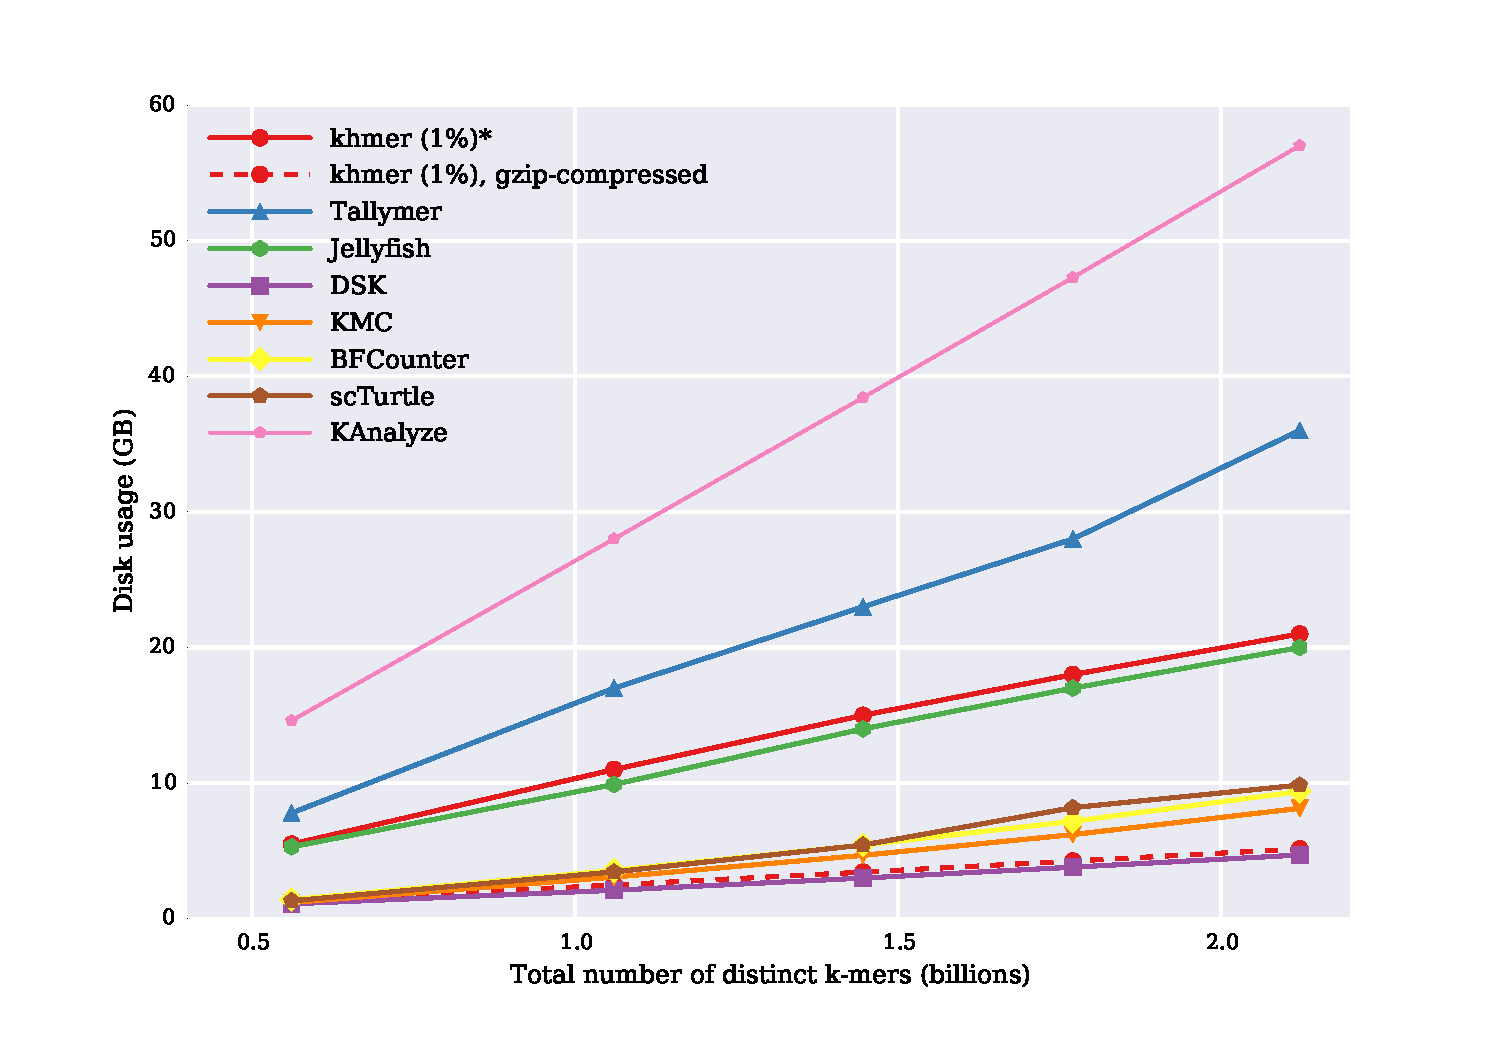
\includegraphics[width=5in]{./figure/disk_benchmark}}
\caption{\bf Disk storage usage of different k-mer counting tools to calculate k-mer 
abundance histograms in GB (y axis),
plotted against the number of distinct k-mers in the data set (x axis).  ($^*$) Note 
that khmer does not use the disk during counting or retrieval, although its hash 
tables can be saved for reuse.}
\label{fig:cmp_disk}
\end{figure}

\begin{figure}[!ht]
\centerline{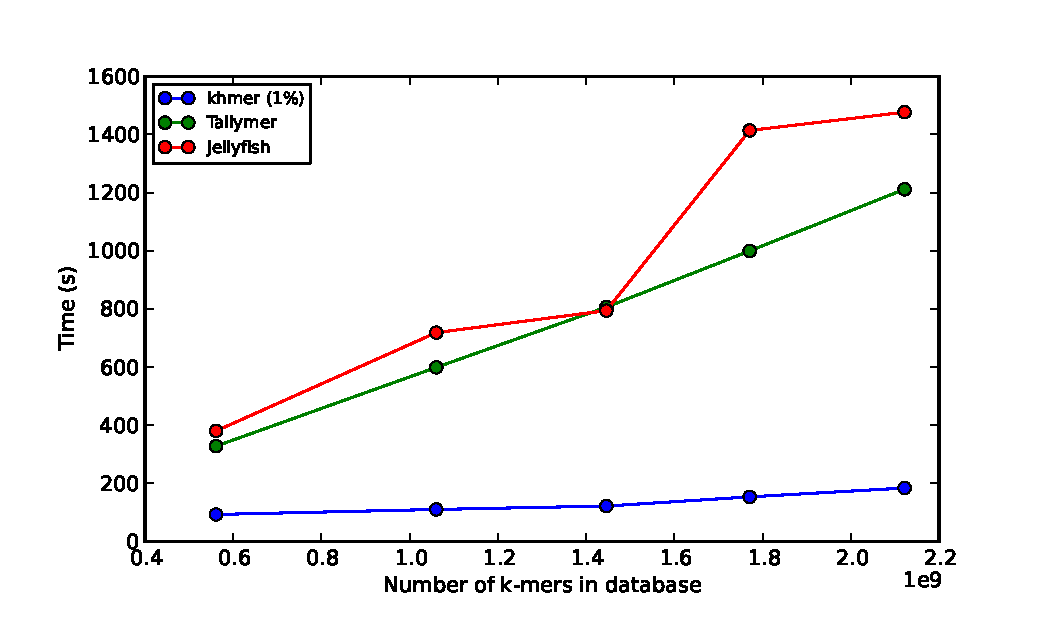
\includegraphics[width=5in]{./figure/count_benchmark}}
\caption{\bf Time for several k-mer counting tools to retrieve the counts of 9.7m randomly 
chosen k-mers (y axis), plotted against the number of unique k-mers in the data set 
being queried (x axis).  DSK does not support this functionality.}
\label{fig:cmp_count}
\end{figure}

\begin{figure}[!ht]
\centerline{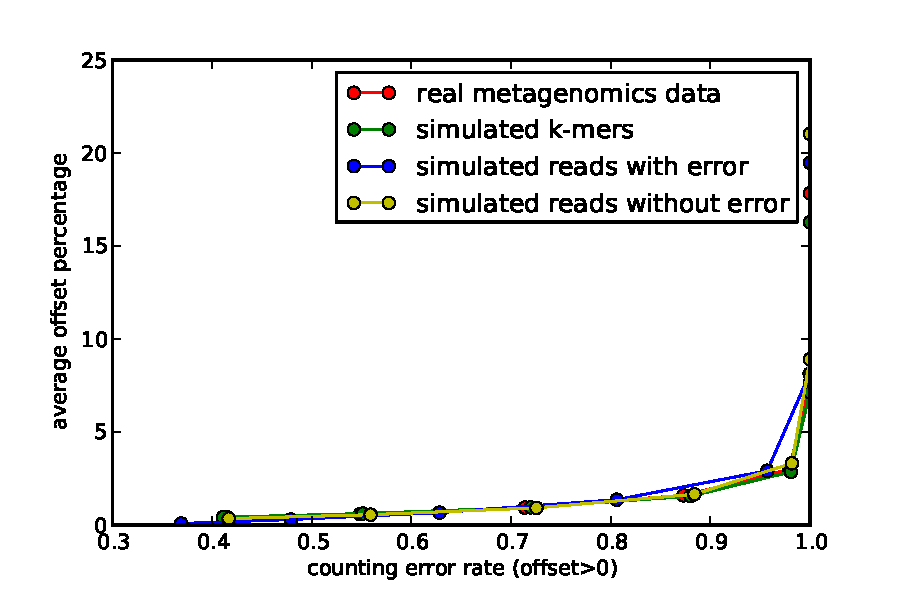
\includegraphics[width=5in]{./figure/average_offset_vs_fpr}}
\caption{\bf Relation between average miscount --- amount by which
the average count for k-mers is incorrect --- on the y axis, plotted against
error rate (x axis), for four data sets.  The four data
sets were chosen to have the same total number of k-mers: one
metagenome data set; a set of randomly generated k-mers; a set
of reads, chosen with 3x coverage and 1\% error, from a randomly generated
genome; and a simulated set of error-free reads (3x) chosen from a randomly
generated genome.}
\label{fig:average_offset_vs_fpr}
\end{figure}

\begin{figure}[!ht]
\centerline{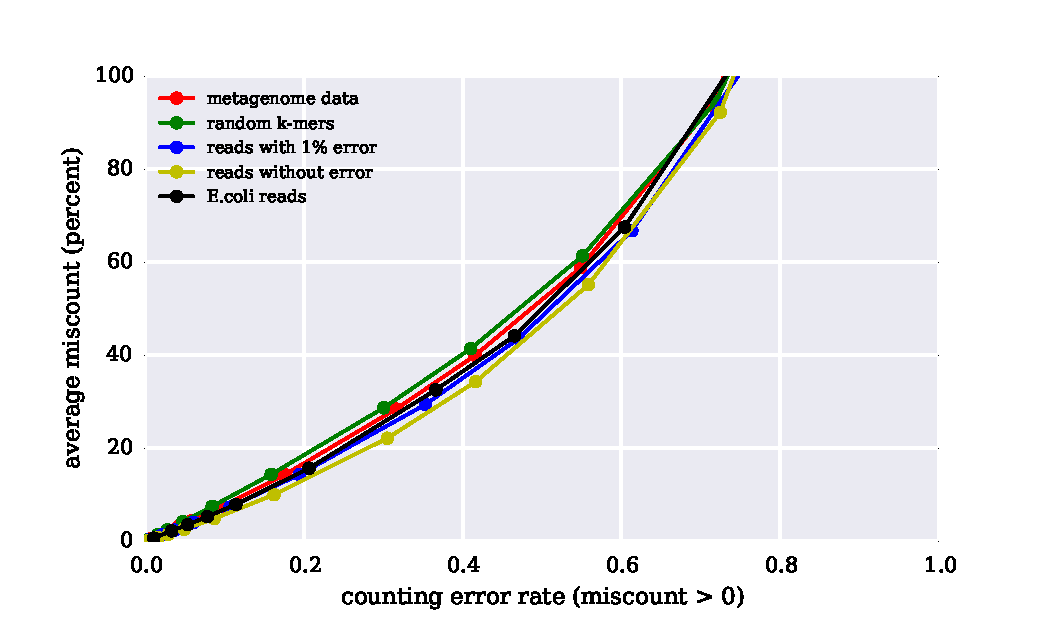
\includegraphics[width=5in]{./figure/percent_offset_vs_fpr}}
\caption{\bf Relation between percent miscount --- amount by which
the count for k-mers is incorrect relative to its true count --- on the y axis, plotted 
against
error rate (x axis), for four data sets.  The four data
sets are the same as in Figure \ref{fig:average_offset_vs_fpr}.}
\label{fig:percent_offset_vs_fpr}
\end{figure}

\begin{figure}[!ht]
\centerline{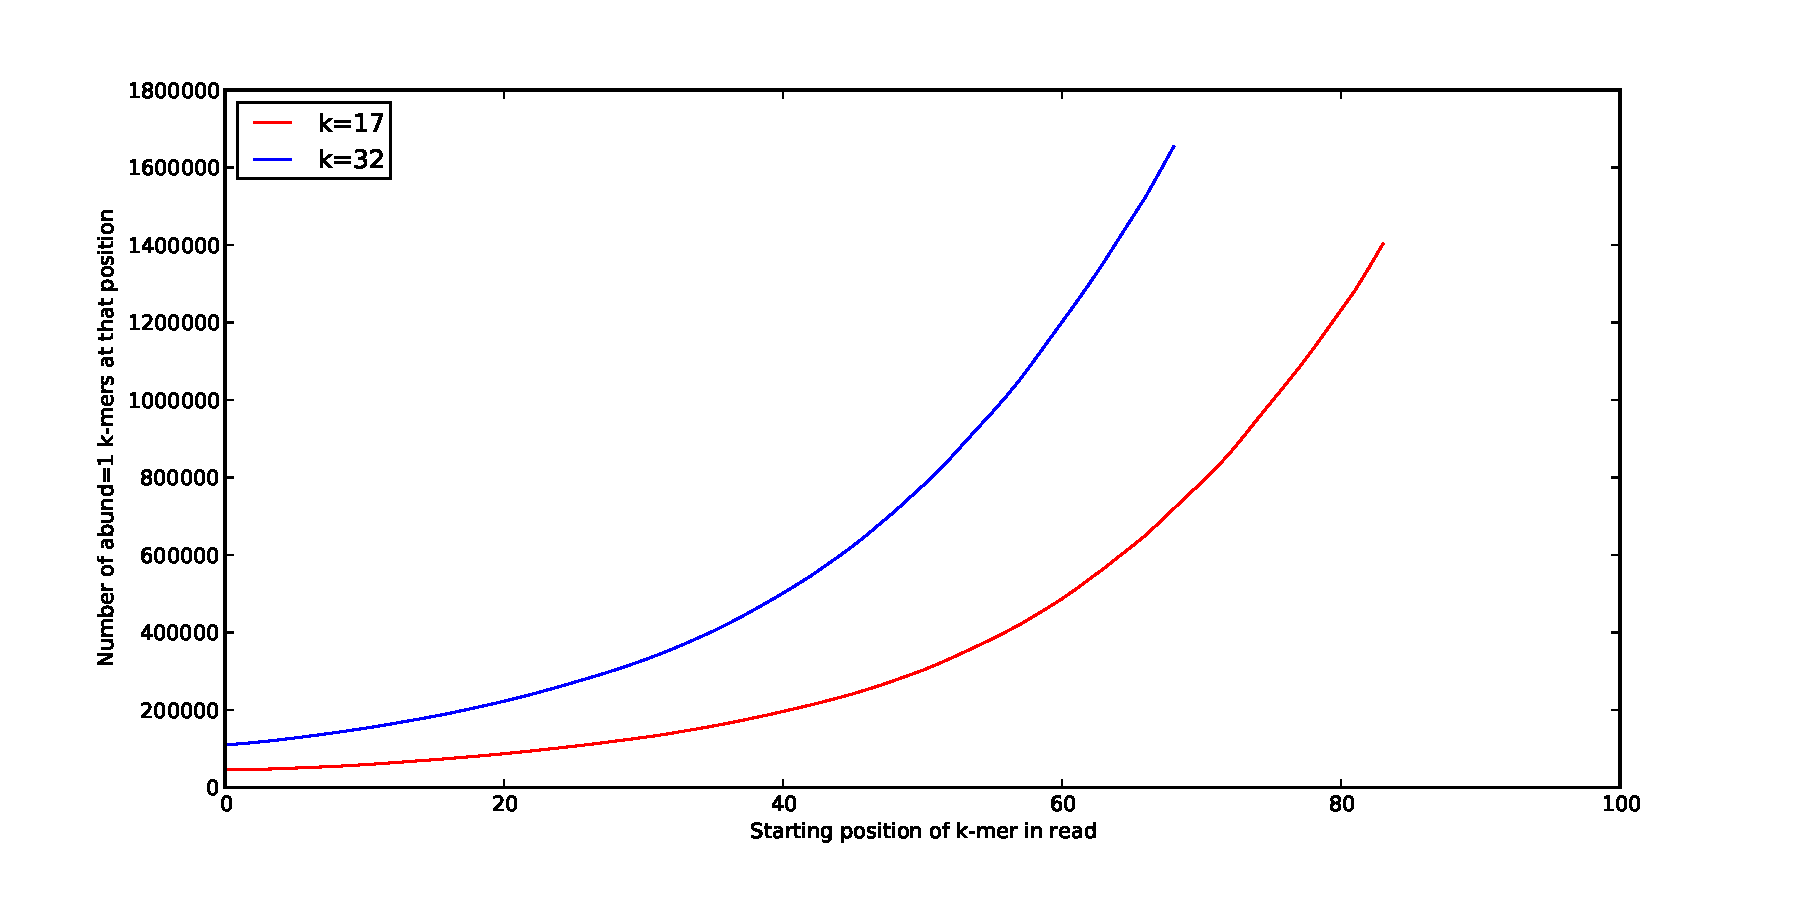
\includegraphics[width=5in]{./figure/perc_unique_pos}}
\caption{\bf Number of unique k-mers (y axis) by starting position within read (x axis) in 
an untrimmed {\em E. coli} 100-bp Illumina shotgun data set, for k=17 and k=32.  The 
increasing numbers of unique k-mers are a sign of the increasing sequencing error 
towards the 3' end of reads.  Note that there are only 69 starting positions for 32-mers 
in a 100 base read.}
\label{fig:perc_unique_pos}
\end{figure}

\clearpage
\section*{Tables}
%\begin{table}[!ht]
%\caption{
%\bf{Table title}}
%\begin{tabular}{|c|c|c|}
%table information
%\end{tabular}
%\begin{flushleft}Table caption
%\end{flushleft}
%\label{tab:label}
% \end{table}

% @CTB fix data set names/descr; caption; reference.
\begin{table}[!ht]
\caption{
\bf{Benchmark soil metagenome data sets for k-mer counting performance, taken from
\cite{Howe2012}.}}
\begin{tabular}{ |c | c |c| c|c| }
Data set & size of file (GB) & number of reads & number of distinct
k-mers & total number of k-mers \\
\hline \\
subset 1        & 1.90 &  9,744,399 &   561,178,082 &   630,207,985 \\
subset 2        & 2.17 & 19,488,798 & 1,060,354,144 & 1,259,079,821 \\
subset 3        & 3.14 & 29,233,197 & 1,445,923,389 & 1,771,614,378 \\
subset 4        & 4.05 & 38,977,596 & 1,770,589,216 & 2,227,756,662 \\
entire data set & 5.00 & 48,721,995 & 2,121,474,237 & 2,743,130,683 \\
\end{tabular}
\begin{flushleft}
\end{flushleft}
\label{table:datasets}
\end{table}

%%%%%%%%%%%%%%%%%%%%%%%

% These numbers are got by running these commands: (to be integrated in Makefile)

% to get number of unique k-mers:
% python bloom_count.py ecoli_ref_head45000.fasta 12 100000000 4
% python bloom_count.py random_kmers_1M_3c.fa 12 100000000 4
% python bloom_count.py random_reads_1.67M_3c_0.03e.fa 12 100000000 4
% python bloom_count.py random_reads_2.54M_3c_0.00e.fa 12 100000000 4
% python bloom_count.py MH0001.trimmed.head176800.fa 12 100000000 4
% 
% to get number of total k-mers:
% number of reads x reads_length -12 + 1
% reads length = 44bp, except ecoli reads = 100 bp


\begin{table}[!ht]
\caption{
\bf{Data sets used for analyzing miscounts.}}
\begin{tabular}{ | p{5cm} | c | c | c |}
Data set & Size of data set file & Number of total k-mers & Number of unique k-mers \\
\hline \\
Real metagenomics reads                                  & 7.01M  & 2,917,200  & 1,944,996 \\
\hline
Totally random reads with randomly generated k-mers      & 3.53M  & 2,250,006  & 1,973,059 \\
\hline
Simulated reads from simulated genome with error         & 5.92M  & 3,757,479  & 2,133,592 \\
\hline
Simulated reads from simulated genome without error      & 9.07M  & 5,714,973  & 1,989,644 \\
\hline
Real {\em E. coli} reads                                        & 4.85M  & 4,004,911  & 2,079,302 \\
\end{tabular}
\begin{flushleft}
\end{flushleft}
\label{table:random_data}
\end{table}



%%%%%%%%%%%%%%%%%%%%%%%

% data in pipeline/ecoli_ref.fastq.ka.r?.fq.out
\begin{table}[!ht]
\caption{
\bf{Iterative low-memory k-mer trimming.  The results of trimming
  reads at unique (erroneous) k-mers from a 165 Mbp short-read data
  set in under 40 MB of RAM.  After each iteration, we measured the
  total number of distinct k-mers in the data set, the total number
  of unique (and likely erroneous) k-mers remaining, and the
  number of unique k-mers present at the 3' end of reads.}}
\begin{tabular}{ | c | c | c | c | c | c |}
iteration & FP rate & bases trimmed & total k-mers & unique k-mers & 
unique k-mers at 3' end \\
\hline \\
untrimmed  &      -  &      - & 28.1m & 22.4m & 43\% \\
1          & 78.1\%  & 22.9\% &  8.2m &  2.8m & 41\% \\
2          &   10\%  &  2.9\% &  5.4m &   95k &  4\% \\
3          &  3.1\%  &  0.2\% &  5.3m &  3.8k &  0\% \\
4          &  3.1\%  &  0.0\% &  5.3m &   230 &  0\% \\
\end{tabular}
\begin{flushleft}
\end{flushleft}
\label{table:loop_trim}
\end{table}


%%%%%%%%%%%%%%%%%%

% data in pipeline/keep*.x.mg*.hist (true k-mers)
% data in pipeline/mg*.x.keep*.hist (total k-mers)
% data in pipeline/keep*.x.mg*.hist (true k-mers)
% @CTB address -2 issue
\begin{table}[!ht]
\caption{
\bf{Low-memory digital normalization. The results of digitally
  normalizing a 5m read {\em E. coli} data set to C=20 with k=20 under
  several memory usage/error rates.  The error rate
  (column 1) is empirically determined.  We measured reads remaining,
  number of ``true'' k-mers that were removed during the normalization
  process, and the number of total k-mers remaining.  Note: at high
  error rates, reads are erroneously removed due to inflation
  of k-mer counts.}}
\begin{tabular}{ | c | c | c | c | c | c |}
memory/FP rate & retained reads & true k-mers removed & retained total k-mers \\
\hline \\
 800 MB/0.0\% & 1,657,065 & 2 &   28m \\
 80 MB/39.3\% & 1,635,326 & 2 & 27.8m \\
 40 MB/82.9\% & 1,592,719 & 2 & 27.4m \\
\end{tabular}
\begin{flushleft}
\end{flushleft}
\label{table:loop_norm}
\end{table}

%%%%%%%%%%%%%%%%%%%%%%%%%%%

% data in *.cover
\begin{table}[!ht]
\caption{
\bf{{\em E. coli} genome assembly after low-memory digital normalization.
  A comparison of assembling reads digitally normalized with low memory/high
  error rates.  The reads were digitally normalized using 3-pass methods  (normalization to C=20, followed by
  low-abundance k-mer trimming, followed by normalization to C=5; see
  \cite{Brown2012} for more information) and were assembled using Velvet.
  We measured total sequence recovered,
  as well as percent of true MG1655 genome covered by the assembly.}}
\begin{tabular}{ | c | c | c | c | c | c |}
memory/FP rate & N contigs & total sequence & \% of true genome covered \\
\hline \\
      800 MB/0.0\% & 617 & 4,571,174 & 99.75\% \\
      80 MB/39.3\% & 613 & 4,570,562 & 99.75\% \\
      40 MB/82.9\% & 612 & 4,570,924 & 99.73\% \\
\end{tabular}
\begin{flushleft}
\end{flushleft}
\label{table:assembly}
\end{table}

% @CTB be sure to explain the tables well!
% @CTB do we talk about how efficiently fp rate drops with incr memory?
% @CTB make point that diginorm/first step is hard.
% @CTB KMC


\end{document}

